% Tikz File 'mytikz.tex'
\documentclass{standalone}
\usepackage{amsmath,xparse}
\DeclareMathOperator{\vsd}{VSD}
\DeclareMathOperator{\asd}{ASD}
\DeclareMathOperator{\ea}{EA}
\DeclareMathOperator{\bb}{BB}
\DeclareMathOperator{\voc}{VC}
\usepackage{tikz}

\pgfdeclarelayer{bg} 
\pgfdeclarelayer{background}
\pgfdeclarelayer{foreground}
\pgfsetlayers{background,main,foreground}
\tikzstyle{sensor}=[draw, text width=2em, 
    text centered, minimum height=2.5em]
 \tikzstyle{s}=[draw, text width=6em, 
    text centered, minimum height=5em]
 \tikzstyle{sim}=[draw, text width=8em, 
    text centered, minimum height=6em]
\tikzstyle{ann} = [above, text width=5em]
\tikzstyle{a} = [sensor, text width=8em,
    minimum height=9em, rounded corners]
 \tikzstyle{v} =[circle, thick, minimum size=0.8cm, draw=black]
  \tikzstyle{vv} =[circle, thick,  dashed,draw=black!50]
  \def\blockdist{2.3}
\def\edgedist{2.5}
\begin{document}
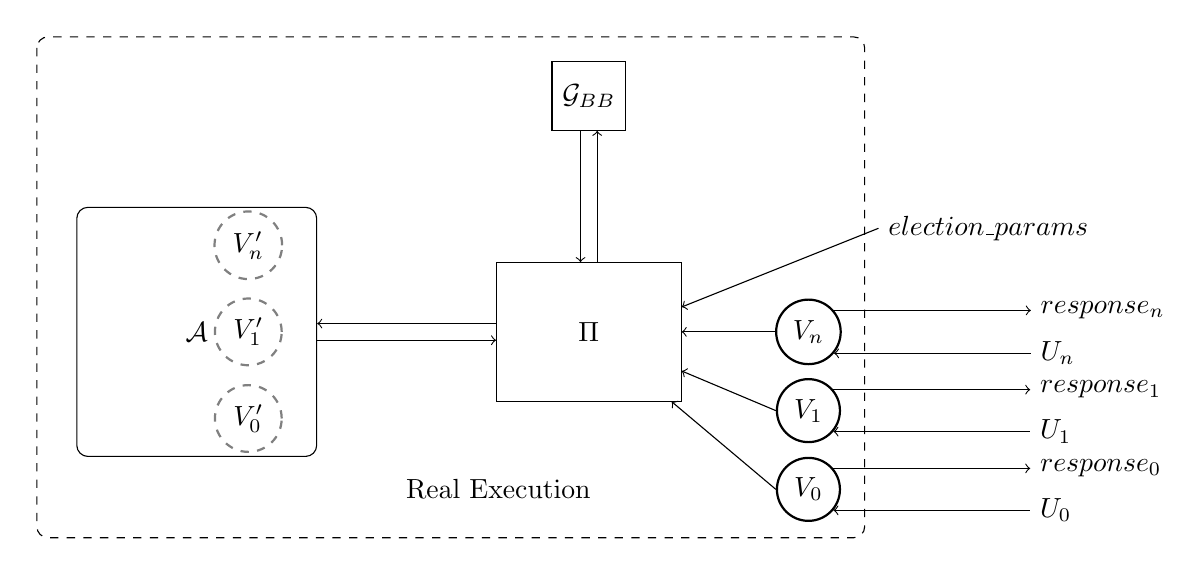
\begin{tikzpicture}
    \node (s) [a] {$\mathcal{A}$};
    \path (s.east)+(1.5*\blockdist,3) node (g) [sensor] {$\mathcal{G}_{BB}$};
    \path (s.east)+(1.5*\blockdist,0) node (system) [s] {$\Pi$};
    \path (system.east) +(0.7*\blockdist,-2) node (v0) [v] {$V_0$};
    \path (system.east) +(0.7*\blockdist,-1) node (v1) [v] {$V_1$};
     \path (system.east) +(0.7*\blockdist, 0) node (vn) [v] {$V_n$};
     \path (s.west) +(0.95*\blockdist,-1.1) node (v0') [vv] {$V_0'$};
      \path (s.west) +(0.95*\blockdist,0) node (v1') [vv] {$V_1'$};
       \path (s.west) +(0.95*\blockdist,1.1) node (vn') [vv] {$V_n'$};
    \path (s.east) +(\blockdist, -2) node (RE) {Real Execution};
    \draw[transform canvas={yshift=0.7ex},->] (system) -- (s);
    \draw[transform canvas={yshift=-0.7ex},<-] (system) -- (s);
    \draw[transform canvas={xshift=0.7ex},->] (system) -- (g);
    \draw[transform canvas={xshift=-0.7ex},<-] (system) -- (g);
     \path [draw, <-] (system) --  (v1.west);
      \path [draw, <-] (system) -- (v0.west);
      \path [draw, <-] (system) --  (vn.west);
    \draw [<-] (v0.-40)-- node [ann] {} + (\edgedist,0) 
        node[right] {$U_0$};
      \draw [<-] (v1.-40)-- node [ann] {} + (\edgedist,0) 
        node[right] {$U_1$};
     \draw [<-] (vn.-40)-- node [ann] {} + (\edgedist,0) 
        node[right] {$U_n$};
     \draw [->] (v0.40)-- node [ann] {} + (\edgedist,0) 
        node[right] {$response_0$};
      \draw [->] (v1.40)-- node [ann] {} + (\edgedist,0) 
        node[right] {$response_1$};
     \draw [->] (vn.40)-- node [ann] {} + (\edgedist,0) 
        node[right] {$response_n$};
        \draw [<-] (system.15) -- node [ann] {} + (\edgedist,1) 
        node[right] {$election\_params$};
    \begin{pgfonlayer}{background}
        \path (s.west |- g.north)+(-0.5,0.3) node (a) {};
        \path (v0.south -| v0.east)+(+0.3,-0.2) node (b) {};
        \path[rounded corners, draw=black, dashed]
            (a) rectangle (b);
    \end{pgfonlayer}
\end{tikzpicture}
\end{document}